\documentclass{../cs-classes/cs-classes}

\title{Information theory and coding}
\author{Bartek Blaszczyszyn\\ Notes by Antoine Groudiev}

\begin{document}
\section*{Introduction}
This document is Antoine Groudiev's class notes while following the class \emph{Théorie de l'information et codage} (Information theory and coding) at the Computer Science Department of ENS Ulm. It is freely inspired by Bartek Blaszczyszyn's class notes. 

This class contains two main parts: information theory, and coding theory. Information theory gives mathematical basis to build a notion of \emph{information quantity}: given a text, how to "weight" the information contained in the sequence of characters? Some languages are more concise, but still provide the same quantity of information. Coding theory aims at finding the most concise way to represent information, with the smallest number of characters. Such theory -- \emph{source coding} -- has many applications (storage, \dots). Another branch of coding is \emph{canal coding} -- allowing "repetition" in a message to avoid the loss of information in a canal.

\section{Entropy and source coding}
We shall introduce \emph{Shannon’s entropy} of a probability distribution on a discrete space and study its basic properties. Our goal is to prove \emph{Shannon’s source coding theorem} formulated in 1948. It will allow us to interpret the entropy as a notion of the \emph{amount of information} "carried" by random variables of a given distribution.

\subsection{Shannon's entropy}
Let $\X$ be a finite or countable set, and $p := \{p(x) \: | \: x\in \X \}$ be a probability distribution on $\mathcal{X}$.

\begin{definition}[Shannon's entropy] We define (Shannon's) entropy $H(p)$ of $p$ to be:
\begin{equation}
    H(p) := -\sum_{x\in\X}p(x)\log p(x)
\end{equation}
with the convention that $0\log 0 = 0$, and $a\log 0 = -\infty$ for $a>0$.
We will later on discuss the base of the logarithm.
\end{definition}

\begin{remark}
    In this mathematical generalisation, $\X$ is the equivalent of a symbol alphabet, and $p$ represents the text. The nature of the elements of $\X$ is not important: the entropy, the average, \dots depend only on $\X$ and on the distribution $p$. Therefore, we can re-label the elements of $\X$.
\end{remark}

\begin{definition}[Entropy of a random variable]
    Let $X$ be a random variable on $\X$ with distribution $p$, that is $\P(X=x) = p(x)$, also denoted $X \sim p$. We define:
    \begin{equation}
        H(X) := H(p) = -\E(\log p(X))
    \end{equation}
\end{definition}

Observe that $0\leq H(p) \leq +\infty$, and that $H(p)=0$ if and only if $X$ is constant almost surely.

\begin{property}
    Entropy is invariant with respect to deterministic injective mapping $f: \X \to \mathcal{Y}$:
    \begin{equation*}
        H(X) = H(f(X))
    \end{equation*}
\end{property}

The entropy $H(p)$ can be interpreted as the \emph{amount of information} carried on average by one realization from the distribution $p$. Later in this chapter, we shall prove a result supporting this interpretation. 

\begin{definition}[Entropy units] The unit of the entropy depends on the \emph{base of the logarithm}:
    \begin{itemize}
        \item In binary basis, when $\log = \log_2$, we denote $H(p)=H_2(p)$, and its unit is the $[bit/symbol]$ (per realization of $X$).
        \item In arbitrary basis $b>0$, when $\log = \log_b$, we denote $H(p)=H_b(p)$, and its unit is the $[b-digit/symbol]$ (a $b$-digit is a digit which can take $b$ values).
        \item In basis $e$, when $\log = \ln$, we denote $H(p)=H_e(p)$, and its unit is the $[nat/symbol]$ (nat is the natural unit of information).
    \end{itemize}
    
    The conversion between units can be done by changing the base of the logarithm:
    \begin{equation*}
        H_b(p) = \frac{H_2(p)}{\log_2(b)}
    \end{equation*}
\end{definition}

\begin{example}[Bernoulli distribution]
    Let $\mathcal{X}=\{0, 1\}$, and $p$ the Bernoulli distribution such as
    \begin{equation*}
        \begin{cases}
            p(0) = p\\
            p(1) = 1 - p
        \end{cases}
    \end{equation*}
    Therefore, we have $H(p)=-p\log(p) - (1-p)\log(1-p)$. The Bernoulli distribution with the maximum entropy is:
    \begin{equation*}
        \max_{0\leq p\leq 1} H_2(p) = H_2(1/2) = 1 \: [bit/symbol]
    \end{equation*}
    % TODO: graph of entropy depending on p
\end{example}

\begin{example}[Uniform distribution]
    Let $\mathcal{X}$ be a finite set, and $p$ the uniform distribution, that is:
    \begin{equation*}
        \forall x\in \X, \: p(x) := \frac{1}{|\X|}
    \end{equation*}
    Therefore, we have $H(p) = \log(|X|)$.
\end{example}

\begin{example}[Geometric distribution]
    Let $\X = \N^\star$ and $p$ the geometric distribution of parameter $p>0$, that is:
    \begin{equation*}
        \forall n\in \N^\star, \: p(n) = p(1-p)^{n-1}
    \end{equation*}
    Recall that $\E[X] = \frac{1}{p}$ when $X$ follows a geometric law of parameter $p$.

    Therefore, we have:
    \begin{equation*}
        H(p) = \log\left(\frac{1-p}{p}\right) - \frac{1}{p}\log(1-p)
    \end{equation*}
\end{example}

\subsection{Gibbs' inequality}
\begin{theorem}[Gibbs' inequality]
    Let $p$ and $q$ be two probability distributions on $\X$. Then:
    \begin{equation}
        \label{eq:gibbs}
        H(p) = -\sum_{x\in\X} p(x)\log p(x)  \leq - \sum_{x\in\X} p(x)\log q(x)
    \end{equation}
    Moreover, if $H(p)<\infty$, then there is equality in \eqref{eq:gibbs} if and only if $p=q$.
\end{theorem}
The right-hand-side of \eqref{eq:gibbs} is called \emph{cross entropy} between $p$ and $q$.

\begin{proof}
    Let $x\sim p$. Gibbs' inequality is equivalent to:
    \begin{equation*}
        \E[\log p(X)] \geq \E[\log q(X)]
    \end{equation*}
    If $\E[\log q(X)] = -\infty$, the inequality is trivial. Otherwise, since we have $\E[\log q(X)] \leq 0$:
    \begin{equation*}
        \begin{aligned}
            \E[\log q(X)] - \E[\log p(X)] &= \E[\log q(X) - \log p(X)] \\
            &= \E\left[\log\left(\frac{q(X)}{p(X)}\right)\right]
        \end{aligned}
    \end{equation*}
    $\log$ being concave, by applying Jensen's inequality, we obtain:
    \begin{equation*}
        \begin{aligned}
            \E\left[\log\left(\frac{q(X)}{p(X)}\right)\right] &\leq \log\E\left[\frac{q(X)}{p(X)}\right] \\
            &= \log\sum_{x\in\X} \frac{q(x)}{p(X)}p(x)\\
            &= \log\sum_{x\in\X} q(x)\\
            &= \log 1 = 0
        \end{aligned}
    \end{equation*}
    The equality in Jensen's inequality holds if and only if $\frac{q(X)}{p(X)}$ is almost surely constant, that is $p=\lambda q$ almost surely; furthermore, we must have $\lambda=1$ since both $p$ and $q$ are distributions, hence $p=q$ almost surely. 
\end{proof}

\begin{corollary}[Uniform distribution maximizes entropy]
    Let $p$ be a probability distribution on some set $\X$ with $|\X|<\infty$. Then:
    \begin{equation*}
        0\leq H(p) \leq \log(|\X|)
    \end{equation*}
    and the equality holds if and only if $p$ is uniform on $\X$.
\end{corollary}

\begin{proof}
    Let $X \sim p$ and be $q$ the uniform distribution on $\X$. By Gibbs' inequality:
    \begin{equation*}
        H(p) \leq -\sum_{x\in\X}p(x)\log\left(\frac{1}{|X|}\right) = \log|X|
    \end{equation*}
    Notice that $\log|X|$ is the entropy of the uniform distribution $q$.
\end{proof}

\begin{corollary}[Geometric distribution maximizes entropy in the set of probability measures on $\N^\star$ having given expectation]
    Let $p$ be a probability distribution on $\X=\N^\star$ with mean $\mu=\sum_{n\geq 1} np(n) < \infty$. Then:
    \begin{equation*}
        H(p)\leq\mu\log(\mu)-(\mu-1)\log(\mu-1)
    \end{equation*}
    where the right-hand-side is the entropy of the geometric distribution with parameter $1/\mu$.
\end{corollary}

\begin{proof}
    Let $p$ be a probability distribution on $\X=\N^\star$ with mean $\mu<\infty$, and $q$ the geometric distribution of parameter $1/\mu$. According to Gibbs' inequality,
    \begin{equation*}
        \begin{aligned}
            H(p)&\leq-\sum_{n\geq 1}p(n)\log q(n) \\
            &=-\sum_{n\geq 1}p(n)\log\left(\frac{1}{\mu}\left(1-\frac{1}{\mu}\right)^{n-1}\right)\\
            &=\sum_{n\geq 1}p(n)\log \mu - \sum_{n\geq 1}(n-1) p(n)\log\left(1-\frac{1}{\mu}\right) \\
            &=\log\mu - \log\left(1-\frac{1}{\mu}\right)\left(\mu - 1\right)\\
            &=\log\mu - \left(\log(\mu-1)-\log\mu\right)\left(\mu - 1\right)\\
            &=\log\mu + \mu\log\mu - \mu\log(\mu-1) + \log(\mu-1) - \log\mu\\
            &=\mu\log\mu - (\mu-1)\log(\mu-1) = H(q)
        \end{aligned}
    \end{equation*}
\end{proof}

\subsection{Entropy of random vectors}
\begin{definition}[Entropy of random vectors]
    Let $X:=(X_1, \dots, X_n)$ be a random vector on $\X=\X_1\times \dots \times \X_n$, for some $n\geq 1$, with distribution
    \begin{equation*}
        p(x_1^n)=p(x_1, \dots, x_n) = \P(X_1=x_1, \dots, X_n=x_n)
    \end{equation*}
    The entropy of $X$ is defined as the entropy of its distribution:
    \begin{equation}
        H(X)=-\sum_{x\in \X}p(x)\log p(x) = -\E[\log p(X)]
    \end{equation}
\end{definition}

\begin{property}[Entropy of independent variables]
    Let $X:=(X_1, \dots, X_n)$ be a vector of \emph{idenpendent}, random variables. Then:
    \begin{equation}
        H(X)=\sum_{i=1}^n H(X_i)
    \end{equation}
\end{property}

\begin{proof}
    Let $p$ be the joint distribution of $X$. By independence, $p(x)=\prod_{i=1}^n p_i(x_i)$. Hence:
    \begin{equation*}
        \begin{aligned}
            H(X)&=-\E[\log p(X)]\\
            &=-\E\left[\log\prod_{i=1}^n p_i(X_i)\right]\\
            &=-\E\left[\sum_{i=1}^n\log p_i(X_i)\right]\\
            &=\sum_{i=1}^n-\E[\log p_i(X_i)]\\
            &=\sum_{i=1}^n H(X_i)
        \end{aligned}
    \end{equation*}
\end{proof}

\begin{property}[Independence maximizes entropy]
    Let $X:=(X_1, \dots, X_n)$ be a vector of (arbitrary) random variables for some $n\geq 1$. Then:
    \begin{equation}
        H(X)\leq \sum_{i=1}^n H(X_i)
    \end{equation}
    Moreover, the equality holds if and only if $X_1, \dots, X_n$ are independent.
\end{property}

\begin{proof}
    By induction. If $n=1$, the results holds. Let $X$ be an $n$-vector of random variables and $X_{n+1}$ another random variable. Denote $q(x, y)=p(x)p_{n+1}(y)$, where $X\sim p$ and $X_{n+1}\sim p_{n+1}$, and $(X_1, \dots, X_n, X_{n+1})\sim p'$. Since:
    \begin{equation*}
        \begin{aligned}
            H(X) + H(X_{n+1}) &= -\E[\log p(X)+\log p_{n+1}(X_{n+1})]\\
            &=-\E[\log q(X, X_{n+1})]\\
            &\geq -\E[\log p'(X, X_{n+1})] = H(X_1, \dots, X_n, X_{n+1})
        \end{aligned}
    \end{equation*}
    by Gibbs' inequality, the property is hereditary. Furthermore, there is equality in Gibbs' when $p'=q$, hence when $X_{n+1}$ is independent from $X$, i.e. when $X_1, \dots, X_n, X_{n+1}$ are independent.
\end{proof}

\subsection{Typical sequences of random variables}
\begin{definition}[Typical sequences]
    Let $\X$ be a set with $D:=|\X|<\infty$, and $X=(X_1, \dots, X_n)\in \X^n$ a vector of independent and identically distributed random variables. Let $p$ be the distribution of $X$ on $\X$, with $p(x)=\prod_{i=1}^n p(x_i)$. We denote $H_D:=H_D(p)=-\E[\log_Dp(X)]$, expressed in $D$-digits/symbol.

    For $\epsilon>0$, the following subset of realizations of $\X^n$
    \begin{equation}
        A_\epsilon^{(n)}:=\left\{x\in \X^n \: : \: \big| -\frac{1}{n}\sum_{i=1}^n \log_Dp(x_i)-H_D\big|\leq \varepsilon\right\}\subseteq \X^n
    \end{equation}
    is called the set of $\epsilon$-typical vectors in $\X^n$ with respect to $p$.

    Intuitively, the typical vectors are the vectors that probabilistically appear a lot, and that we need to represent faithfully.
\end{definition}

\begin{remark}
    \begin{equation*}
        \E\left[-\frac{1}{n}\sum_{i=1}^n \log_Dp(X_i)\right] = \E[-\log_Dp(X)]=H_D
    \end{equation*}
    and, by the Law of Large Numbers (LNN for short):
    \begin{equation*}
        \lim_{n\to+\infty}-\frac{1}{n}\sum_{i=1}^n \log_Dp(X_i) = \E[-\log_D p(X)] = H_D
    \end{equation*}
    We shall see that the probability distribution of $X$ concentrates on the set of typical sequences, and, dependending on the entropy $H_D$, the dimension of this set can be smaller than $n$ (the dimension of the whole space $\X^n$).
\end{remark}

\begin{property}[Typical sequences concentrate probability]
    \label{prop:typ-seq-concentrate}
    Let $X=(X_1, \dots, X_n)$ be a vector of i.i.d. random variables, with $X_i\sim p$ on $\X$, and $D:=|\X|<\infty$. We have:
    \begin{equation}
        \label{eq:lim-p-1}
        \lim_{n\to+\infty}\P(X\in A_\epsilon^{(n)})=1
    \end{equation}
    and
    \begin{equation}
        \label{eq:card-A}
        |A_\epsilon^{(n)}|\leq D^{n(H_D+\epsilon)}
    \end{equation}
    \begin{figure}
        \center
        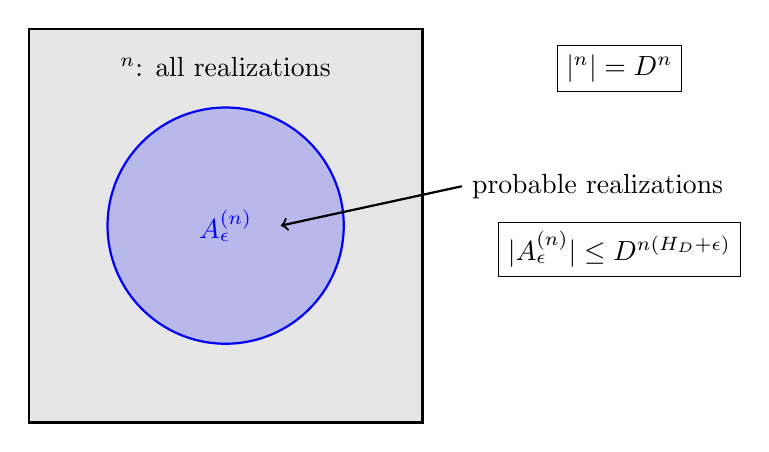
\begin{tikzpicture}
            \draw [thick, fill=gray, fill opacity=0.2, text opacity=1] (0, 0) rectangle (5, 5) node [above=50pt, pos=0.5] {$\X^n$: all realizations};
            \draw [thick, color=blue, fill=blue, fill opacity=0.2, text opacity=1] (2.5, 2.5) circle[radius=1.5] node [color=blue] {$A_\epsilon^{(n)}$};
            \draw [thick, <-] (3.2, 2.5) -- (5.5, 3) node [right] {probable realizations};
            \node[draw] at (7.5, 4.5) {$|\X^n|=D^n$};
            \node[draw] at (7.5, 2.2) {$|A_\epsilon^{(n)}|\leq D^{n(H_D+\epsilon)}$};
        \end{tikzpicture}
        \caption{Representation of $A_\epsilon^{(n)}$}
    \end{figure}
\end{property}

\begin{proof}
    \eqref{eq:lim-p-1} follows from the LLN. For \eqref{eq:card-A}, observe that:
    \begin{equation*}
        \begin{aligned}
            x\in A_\epsilon^{(n)}\implies& -\sum_{i=1}^n \log_D p(x_i)\leq n(H_D+\epsilon)\\
            \iff&\log_D\left(\prod_{i=1}^n p(X_i)\right)\geq -n(H_D+\epsilon)\\
            \iff&\log_Dp(x)\geq -n(H_D+\epsilon)\\
            \iff&p(x)\geq D^{-n(H_D+\epsilon)}
        \end{aligned}
    \end{equation*}
    and since:
    \begin{equation*}
        \begin{aligned}
            1\geq \P(X\in A_\epsilon^{(n)})&=\sum_{x\in A_\epsilon}p(x)\\
            &\geq |A_\epsilon^{(n)}|D^{-n(H_D+\epsilon)}
        \end{aligned}
    \end{equation*}
    which completes the proof.
\end{proof}

\begin{property}[$A_\epsilon^{(n)}$ is the smallest set concentrating probability]
    \label{prop:a-eps-smallest}
    Under the assumptions of Property \ref{prop:typ-seq-concentrate}, let $B\subseteq \X^n$ and $R>0$ such that
    \begin{equation*}
        \lim_{n\to+\infty}\P(X\in B)=1
    \end{equation*}
    and
    \begin{equation*}
        |B|\leq D^{nR}
    \end{equation*}
    Then $R\geq H_D$, that is that $A_\epsilon^{(n)}$ is the smallest set concentrating probability.
\end{property}

\begin{proof}
    Let $\epsilon>0$, and assume $D>1$, otherwise the result is trivial. Observe that:
    \begin{equation*}
        \begin{aligned}
            x\in A_\epsilon^{(n)}\implies&-\sum_{i=1}^n \log_D p(X_i)\geq n(H_D-\epsilon)\\
            \iff& p(x)\leq D^{-n(H_D-\epsilon)}
        \end{aligned}
    \end{equation*}
    Therefore,
    \begin{equation*}
        \begin{aligned}
            \P(X\in A_\epsilon^{(n)}\cap B)&\leq |B|D^{-n(H_D\epsilon)}\\
            &\leq D^{-n(H_D-R-\epsilon)}
        \end{aligned}
    \end{equation*}
    Since $D>1$ and $\lim_{n\to+\infty}\P(X\in A_\epsilon^{(n)}\cap B)=1$, we must have $H_D-R-\epsilon\leq 0$, meaning that $H_D-\epsilon\leq R$. We complete the proof by letting $\epsilon\to 0$. 
\end{proof}

\subsection{Entropy and source coding rate -- Shannon's first theorem}
\begin{definition}[Encoding and decoding]
    Let $X^n=(X_1, \dots, X_n)$ be a vector of i.i.d. random variables, with $X_i\sim p$ on $\X$. We call $X_i$ \emph{source symbols}, and the vector $X^n$ of $n$ source symbols is a \emph{source message} (or \emph{source word}, or \emph{block of source symbols}). 

    Our goal is to \emph{encode} the source message $X^n$ consisting of $n$ symbols using some (hopefully smaller) number of symbols in $\X$. That is, to represent $X^n$ via a function $Y^m=c^{(n)}(X^n)\in \X^m$ for some $m\leq n$, in such a way that one can recover $X^n$ from $Y^m$ via a \emph{decoding function} $d^{(n)}$ at least with high probability.
\end{definition}

\begin{definition}[Compression rate]
    The following ratio $R$ is called \emph{(sources) compression rate}:
    \begin{equation}
        \label{eq:compression-rate}
        R:=\frac{m}{n}
    \end{equation}
\end{definition}

\begin{definition}[Error probability]
    We define the \emph{error probability} $P_e^{(n)}$ to be:
    \begin{equation}
        P_e^{(n)}:=\P\left(d^{(n)}\left(c^{n}(X^n)\right)\neq X^n\right)
    \end{equation}
    which is nothing but the probability that the decoded message is different from the source message.
\end{definition}

\begin{theorem}[Source coding theorem -- Shannon's first theorem (1948)]
    \label{th:shannon-first}
    Let $X^n\in \X^n$ be a vector of i.i.d. random variables, with $X_i\sim p$ on $\X$. Denote $D:=|\X|$ with $1<D<\infty$. Then:
    \begin{equation}
        \label{eq:shannon-ft-1}
        \forall R>H_D(p), \quad \begin{cases}
            \exists c^{(n)}:\X^n\to \X^{\lceil nR\rceil} \\
            \exists d^{(n)}:\X^{\lceil nR\rceil}\to \X^n
        \end{cases}\: \textnormal{such that}\: \lim_{n\to+\infty}P_e(n)=0
    \end{equation}
    Furthermore,
    \begin{equation}
        \label{eq:shannon-ft-2}
        \forall R<H_D(p), \quad \begin{cases}
            \forall c^{(n)}:\X^n\to \X^{\lceil nR\rceil} \\
            \forall d^{(n)}:\X^{\lceil nR\rceil}\to \X^n
        \end{cases}\: \textnormal{we have}\: \lim_{n\to+\infty}P_e(n)>0
    \end{equation}
\end{theorem}

\begin{proof}
    Let's start by proving \eqref{eq:shannon-ft-1}. Let $R>H(p)$ and consider $0<\epsilon<R-H_D(p)$. For $n\geq1$, let $A_\epsilon^{(n)}$ be the set of $\epsilon$-typical sequences for the distribution $p$, and let $f^{(n)}$ be an injection of $A_\epsilon^{(n)}$ into $\X^{\lceil nR\rceil}$. Notice that such an injection exists by \eqref{eq:card-A}.

    Let $x_\star\in X^{\lceil nR\rceil}\setminus f^{(n)}(A_\epsilon^{(n)})$ arbitrary. Such an $x_\star$ exists since the inequality is strict in \eqref{eq:card-A} (we have $H_D+\epsilon<R$). We define the following coding function:
    \begin{equation*}
        c^{(n)}:=x\to \begin{cases*}
            f^{(n)}(x) & for $x\in A_\epsilon^{(n)}$\\
            x_\star & otherwise
        \end{cases*}
    \end{equation*}
    As a decoding function, consider the inverse of $f^{(n)}$ on its image $f^{(n)}(A_\epsilon^{(n)})$, completed arbitrarily on the whole domain $\X^{\lceil nD\rceil}$, that is:
    \begin{equation*}
        d^{(n)}:=x\to\begin{cases*}
            \left[f^{(n)}\right]^{-1}(x) & if $x\in f^{(n)}(A_\epsilon^{(n)})$ \\
            x_0 & otherwise
        \end{cases*}
    \end{equation*}
    for some arbitrary $x_0\in \X^n$. Finally, note that:
    \begin{equation*}
        P_e^{(n)}\leq \P(X\notin A_\epsilon^{(n)})
    \end{equation*}
    Therefore, \eqref{eq:shannon-ft-1} follows from \eqref{eq:lim-p-1}.

    The second statement, \eqref{eq:shannon-ft-2}, follows from Property \ref{prop:a-eps-smallest} considering the set:
    \begin{equation*}
        B:=\{x \:|\: d^{(n)}\left(c^{n}(x)\right) = x\}
    \end{equation*}
\end{proof}

\begin{remark}[Achievable compression rates]
    The source coding theorem -- Theorem \ref{th:shannon-first} -- says that independent $D$-symbols emitted by a source with distribution $p$ can be encoded asymptotically without errors using $H_D(p)$ encoding symbols per sources symbol. Note that
    \begin{equation*}
        H_D(p)\leq H_D(u)=\log_D(D)=1
    \end{equation*}
    where $u$ is the uniform distribution. The zero-error probability is approached asymptotically when increasing the length of the encoding blocks of source symbols.
\end{remark}

\begin{remark}[Source coding rates]
    In general, one may use different sets of coding symbols $\mathcal{Y}$, having arbitrary number $b:=|\mathcal{Y}|>1$ of elements (set of $b$-digits) together with some coding and decoding functions:
    \begin{equation*}
        \begin{cases}
            c^{(n)}:\X^n\mapsto \mathcal{Y}^{n''}\\
            d^{(n)}:\mathcal{Y}^{n''}\mapsto \X^n
        \end{cases}
    \end{equation*}
    In this more general scheme, the ratio:
    \begin{equation}
        R_s:=\frac{\textnormal{number of $b$-digits used to encode one source message}}{\textnormal{number of source symbols in one source message}} = \frac{n''}{n}
    \end{equation}
    is called \emph{(source) coding rate}. It is expressed in $b$-digits/(source) symbol. Considering a bijective mapping $\X^{n'}\mapsto \mathcal{Y}^{n''}$ with $n'$, $n''$ such that $D^{n'}=b^{n''}$ in conjunction with Shannon's first theorem, it is straightforward to see that
    \begin{equation*}
        H_D(p)\log_bD = H_b(p) \: \textnormal{[$b$-digit/(source) symbol]}
    \end{equation*}
    is the \emph{infimum of coding rates over asymptotically error-free source coding}.
    \begin{figure}[!ht]
        \center
        \begin{tikzpicture}
            \draw[->, very thick] (0, 0) -- (10, 0) node [below] {$R_s$ [bit/symbol]};
            \draw[thick] (5, 0.3) -- (5, -0.3) node [below] {$H_2(p)$};
            \fill (0, 0) circle[radius=0.07] node [below] {$0$};

            \fill [pattern=north east lines, pattern color=red] (0, 0) rectangle (5, 0.5) node [above=5pt, pos=0.5, color=red, text width=4cm, align=center] {no error-free source coding};
            \fill [pattern=north east lines, pattern color=green] (5, 0) rectangle (9.9, 0.5) node [above=5pt, pos=0.5, color=green, text width=5cm, align=center] {$\exists$ asymptotically error-free source coding};

        \end{tikzpicture}
        \caption{Source coding "phase transition"}
    \end{figure}
\end{remark}

\section{Uniquely decipherable codes}
We shall introduce some error-free source coding schemes and prove
that in this class the entropy still indicates the infimum of achievable coding rates. The price to pay for error-free coding is \emph{variable code-word length}. The main tool is Kraft's code proposed in 1949.

\subsection{Uniquely decipherable and prefix-free codes}
In the following, we let $\X$ be a finite set of \emph{source symbols}, and $\A$ a set of coding symbols, called \emph{alphabet}. We define $D:=|\A|\in\N^\star$. Note that in general, $D\neq|\X|$. We denote $\A^\star$ the set of \emph{words}, i.e. the finite (including null) sequences of character over alphabet $\A$. We denote $x*y$ or simply $xy$ the concatenation between words $x$ and $y$.
% Concatenation definition

\begin{definition}[Code]
    A \emph{code} $c$ encoding source symbols $\X$ in alphabet $\A$ is a function
    \begin{equation*}
            c: \X\to \A^\star\setminus\{\epsilon\}
    \end{equation*}
    $c(x)$ is called \emph{code-word} of the source symbol $x$, and $l(x):=l(c(x))$ is the \emph{code-word length}. The image of $\X$ by $c$, i.e. the set of all possible code-words, is called \emph{codebook}.
\end{definition}
In general, efficient codes will have code-words with variable length, with more probable source symbols having short code-words. In order to be able to uniquely decode a sequence of source symbols, we require more than just the injectivity of $c$.

\begin{definition}[Codes uniquely decipherable (UD)]
    A code $c: \X\to\A^\star$ is \emph{uniquely decipherable} (UD) if $\forall k, l \geq 1, \forall x_1\dots x_k\in \X, \forall y_1, \dots, y_k\in \X$,
    \begin{equation*}
        c(x_1)*\dots*c(x_k)=c(y_1)*\dots*c(y_k) \implies k=l \land \forall i, x_i=y_i
    \end{equation*}
\end{definition}

\begin{remark}
    Note that $c$ is UD if the following mapping is injective:
    \begin{equation*}
        \begin{aligned}
            X^\star&\to\A^\star\\
            (x_1, \dots, x_n)&\mapsto c(x_1) * \dots * c(x_n)
        \end{aligned}
    \end{equation*}
\end{remark}

\begin{definition}[Prefix-free (PF) codes]
    A code $c: \X\to\A^\star$ is \emph{prefix-free (PF)} if
    \begin{equation*}
        \nexists x\neq y\in \X, \exists a\in\A^\star,\: c(x)*a=c(y)
    \end{equation*} 
    When such an $a\in\A^\star$ exists, $c(x)$ is said to be a \emph{prefix} of $c(y)$.
\end{definition}

\begin{lemma}[PF$\implies$ UD]
    A prefix-free code is uniquely decipherable.
\end{lemma}

\begin{proof}
    Let $c$ be a PF code. Suppose by contradiction that $x_1, \dots, x_k, y_1, \dots, y_l$ violate the UD condition. Let $i$ be the smallest index such that $x_i\neq y_i$. Then, $c(x_i)$ is a prefix of $c(y_i)$ or the other way around, depending on the code length.
\end{proof}

\begin{remark}[Decoding v. sequential decoding of block messages]
    There is a difference between the decoding of UD and PF codes:
    \begin{itemize}
        \item A UD code allows one to uniquely decode, that is to find, given a concatenation $(a_1, \dots, a_n)$ of some code-words, the sequence of symbols $x_i$ for $1\leq i\leq n$ such that
        \begin{equation*}
            c(x_1)*\dots *c(x_n)=(a_1, \dots, a_n)
        \end{equation*} 
        \item A PF code allows one to decode the symbols $x_i$ sequentially, by decoding with $c$ the successive shortest prefixes of the encoded sequence found in the codebook. Sequential decogin simplifies decoding of blocks of symbols. As we shall see, it does not restrict the achievable performance of source coding.
    \end{itemize}
\end{remark}

\begin{example}
    Let's consider codes $c: \X=\{1, 2, 3, 4\} \to \{0, 1\}^\star$. We define:
    \begin{itemize}
        \item A PF hence UD code of constant length, such that
        \begin{equation*}
            c(1) = (0, 0), c(2) = (0, 1), c(3) = (1, 0), c(4) = (1, 1)
        \end{equation*}
        \item A PF hence UD code of variable length
        \begin{equation*}
            c(1) = (0), c(2) = (1, 0), c(3) = (1, 1 0), c(4) = (1, 1, 1)
        \end{equation*}
        \item A not UD hence not PF code:
        \begin{equation*}
            c(1) = (0), c(2) = (1), c(3) = (1, 0), c(4) = (1, 1)
        \end{equation*}
        We have for instance that $c(2)*c(1)=c(3)$ and $c(2)*c(2)=c(4)$.
    \end{itemize}
\end{example}

\begin{property}
    There exists codes that are UD but not PF.
\end{property}

\subsection{Codes on trees}
\begin{definition}[$k$-ary tree]
    For $k\in\N^\star$, a \emph{$k$-ary tree} is a rooted tree in which each node (vertex) has no more than $k$ children. A node of a $k$-ary tree having no children is called a \emph{leaf}; otherwise, it is called an \emph{intermediate node}. A tree in which each node has exactly $k$-children is called an \emph{entire $k$-ary tree}, and is hence an infinite tree with no leaf.
\end{definition}

\begin{remark}
    There is a natural bijection between the set of words $\A^\star$ expressed in the $D$-elements alphabet $\A$, and the vertices of the entire $D$-ary tree. Bearing in mind this bijection, we shall often identify this set of vertices with $A\star$. In particular, the empty word $\epsilon$ is identified with the root of the tree.
    % Graph

    Using the above bijection, a code $c:\X\to\A^\star$ can be seen as a mapping from $\X$ to the nodes of the entire $D$-ary tre.
\end{remark}

\begin{definition}[Coding tree]
    The minimal subtree of the entire $D$-ary tree containing the root and the code-words of the code $c$ is called the \emph{coding tree of $c$}.

    Note that the coding tree is finite since $|\X|<\infty$, and that the leaves of the coding tree are necessarily the code-words of $c$, but some intermediate nodes might also be code-words.
\end{definition}

\begin{lemma}[PF coding trees]
    Code $c$ is PF if and only if it is injective, and it does not have code-words at the intermediate nodes in its coding tree.
\end{lemma}

\begin{figure}[!ht]
    \center
    \begin{tikzpicture}[->]
        \node (tree) {$\epsilon$}
            child { node {(1)} 
                child { node {(1, 1)} }
                child { node {(1, 2)} }
                child { node {\dots} }
                child { node {(1, D)} }
            }
            child { node {\dots} }
            child { node {\dots} }
            child { node {\dots} }
            child {node {(D)} 
                child { node {(D, 1)} }
                child { node {(D, 2)} }
                child { node {\dots} }
                child { node {(D, D)} }
            };
        \node [below=4cm] {\dots};
    \end{tikzpicture}
    \caption{The entire $D$-ary tree}
\end{figure}

A useful equivalent characterization of PF codes involve subtrees of the entire regular tree. For any $w\in\A^\star$, denote by $\mathcal{T}(w)$ the subset of elements of $\A^\star$ for which $w$ is a prefix. In graph representation, $\mathcal{T}(w)$ corresponds to the subtree rooted at $w$ and consisting of all its descendants in the entire $|\A|$-regular tree.

\begin{lemma}[PF and subtrees]
    A code $c$ is PF if and only if the subtrees of the entire regular tree rooted at the code-words corresponding to distinct source symbols are mutually disjoint:
    \begin{equation*}
        \forall x\neq y\in \X, \mathcal{T}(c(x))\cap\mathcal{T}(c(y))=\emptyset
    \end{equation*}
\end{lemma}

\begin{proof}
    $\implies$
    Assume $x\neq y\in\X$ and $a\in \mathcal{T}(c(x))\cap\mathcal{T}(c(y))\neq\emptyset$. Then both $c(x)$ and $c(y)$ are prefixes of $a$, and hence the shorter code-word of the two is a prefix of the longer one.

    $\impliedby$ If $c(x)$ is a prefix of $c(y)$ then $\mathcal{T}(c(y))\subseteq \mathcal{T}(c(x))$, hence the intersection is not empty.    
\end{proof}

\begin{example}[Uniform coding on the full binary tree]
    Assume $|\X|=2^m$ for some $1\leq m<\infty$, $\A=\{0, 1\}$. All elements of $\X$ can be encoded by the vertices of the $m$-th generation of the binary tree, or, equivalently, by the binary sequences of length $m$.

    \begin{figure}[!ht]
        \center
        \begin{tikzpicture}[->]
            \node (tree) {$\epsilon$}
                child { node {(0)} 
                    child { node {\dots} 
                        child { node {(0, \dots, 0)} }
                        child { node {\dots} }
                    }
                    child [missing]
                    child { node {\dots} 
                        child { node {\dots} }
                        child { node {(0, \dots, 1)} }
                    }
                }
                child [missing]
                child [missing]
                child [missing]
                child {node {(1)} 
                    child { node {\dots} 
                        child { node {\dots} }
                        child { node {\dots} }
                    }
                    child [missing]
                    child { node {\dots} 
                        child { node {\dots} }
                        child { node {(1, \dots, 1)} }
                    }
                };
            \draw[thick, -, decoration={brace,mirror},decorate]
                (-6.1, -4.8) -- node[below=5pt] {$2^m = |\X|$} (6.1, -4.8);
        \end{tikzpicture}
        \caption{Binary sequences}
    \end{figure}

    Since the mapping is bijective and all code-words are equal, this is a PF and hence UD code.

    The source coding rate is
    \begin{equation*}
        R_s=\frac{\textnormal{number of bits}}{\textnormal{one source symbol}} = \frac{m}{1} = \log_2|\X| = H_2(\textnormal{uniform}(\X))
    \end{equation*}
    which corresponds to the infimum achievable coding rate when the source symbols are independently, uniformly sampled in $\X$. By Shannon's source coding theorem we cannot do better even accepting only asymptotically error-less coding.
\end{example}

A remaining question is that in case of independent source symbols sampled from some general distribution $p$ on $\X$, how to achieve rates $R_S>H_2(p)$ with error-free (UD, PF) codes? The idea is to encode elemnts of $\X$ using binary sequences of \emph{variable length}, with more likely source symbols having shorter code-words.

\subsection{Kraft's inequality}
Kraft's inequality will be our main tool in studying the performance of UD and PF codes.

\begin{definition}[Aggregated block codes]
    For a code $c$ and $n\in \N^\star$, the corresponding \emph{aggregated block code} $c^{(n)} : \X^n\to \A^\star$ of block-length $n$ is defined as follows:
    \begin{equation*}
        \forall x\in \X^n, c^{(n)}(x) := c(x_1) * \dots * c(x_n)
    \end{equation*}
\end{definition}

\begin{lemma}
    If $c$ is UD then the aggregated block code $c^{(n)}$ is UD.
\end{lemma}

% TODO: proof

\begin{theorem}[Kraft's inequality]
    Let $c$ be a code encoding source symbols $\X$ with alphabet $\A$. Assume $D:=|\A|<\infty$. 
    \begin{enumerate}
        \item If $c$ is UD then
        \begin{equation}
            \label{eq:kraft-ineq}
            \sum_{x\in\X} D^{-l(c(x))}\leq 1
        \end{equation}

        \item Let $\{l(x)\: |\:x\in\X\}$ be a collection of non-negative integers. If
        \begin{equation*}
            \sum_{x\in\X} D^{-l(c(x))}\leq 1
        \end{equation*}
        then there exists a PF (hence UD) code $c$ with code-word lengths $l(x)=l(c(x))$.
    \end{enumerate}
\end{theorem}

\begin{proof}[Proof of Case 1.]
    Assuming $|X|<\infty$ consider UD code $c$ and denote by $l_{\max}$ its maximal code-word length:
    \begin{equation*}
        l_{\max}=\max_{x\in\X} l(c(x)) <\infty
    \end{equation*}
    Let $n\in\N^\star$. Consider the aggregated block code $c^{(n)}$ corresponding to $c$. Recall from the preceding lemma that $c^{(n)}$ is UD. Denote by $\alpha(k)$ the number of code-words of $c^{(n)}$ of length $k$:
    \begin{equation*}
        \alpha(k) := |\{x\in\X \: | \: l(c^{(n)}(x)) = k\}|
    \end{equation*}
    Note that $\alpha(k)=0$ for $k=0$ and for $k>nl_{\max}$. In general $\alpha(k)\leq D^k$, since $c^{(n)}$ is UD and there are at most $D^k$ differen code-words of length $k$.

    We have
    \begin{equation*}
        \begin{aligned}
            \left(\sum_{x\in\X} D^{-l(c(x))}\right)^n &= \sum_{x\in\X} D^{-l(c(x_1)+\dots+c(x_n))}\\
            &= \sum_{x\in\X} D^{-l(c^{(n)}(x))}\\
            &= \sum_{k} \alpha(k)D^{-k}\\
            &\leq \sum_{k=1}^{nl_{\max}} D^kD^{-k}\\
            &= nl_{\max}
        \end{aligned}
    \end{equation*}

    Consequently,
    \begin{equation*}
        \sum_{x\in\X} D^{-l(c(x))} \leq (nl_{\max})^{1/n} \to_{n\to\infty} 1
    \end{equation*}
    which completes the proof of the first statement for $|\X|<\infty$.

    If $|\X|=\infty$, consider an increasing sequence of subsets $\X_m$ such that $\bigcup_m \X_m = \X$ and codes truncated to $\X_m$.
\end{proof}

\begin{proof}[Proof of Case 2.]
    We assume that $|\X|<\infty$. WLOG, let $\X=\{1, \dots, |\X|\}$, chosen such that $l(1)\leq\dots\leq l(|\X|)$. Define $m:=l(|\X|)=\max_{x\in\X} l(x)$. We construct a code $c$ with code-word lengths $l(c(i))=l(i)$ by encoding messages with some vertices of the entire $D$-ary tree as follows (recall $D:=|\A|$):
    \begin{itemize}
        \item The code-word of $1\in\X$ is corresponds to the most recent common ancestor of the lexicographically first group of $D^{m-l(1)}$ on the $m$-th generation.
        \item By the induction, the code-word of $i\in\X$ corresponds to the most recent common ancestor of the lexicographically $i$-th group of $D^{m-l(i)}$ nodes of the $m$-th generation.
    \end{itemize}
    % Graph

    Note that by the assumption of the second statement,
    \begin{equation*}
        \sum_{i=1}^{|\X|}D^{m-l(i)} \leq D^m
    \end{equation*}
    and thus the above construction can be completed. By the construction, subtrees rooted at the selected code-words are disjoint, $\mathcal{T}(c(i)\cap\mathcal{T}(c(j)))=\emptyset$ for $1\leq i\neq j\leq |\X|$, hence by lemma, the constructed code is PF.
    
    We can similarly extend this to the case where $|\X|=\infty$.
\end{proof}

\subsection{Kraft's code}
We have suggested that an efficient UD code has in general variable length of the code-words. Its coding rate can be defined asymptotically on a sequence of source symbols $X_1, X_2, \dots$
\begin{equation}
    \label{eq:compression-infinite}
    R_s := \lim_{n\to\infty} \frac{l(c(X_1))+\dots+l(c(X_n))}{n} \quad \left[\frac{D-\textnormal{digit}}{\textnormal{source symbol}}\right]
\end{equation}
assuming that the limit exists, thus extending the previous definition of $R$ \eqref{eq:compression-rate} for fixed length codes.

For $X_1, X_2, \dots$ i.i.d. with $X\sim p$, by the LLN, the limit in \eqref{eq:compression-infinite} exists a.s. and
\begin{equation*}
    R_s = \E[l(c(X))]
\end{equation*}
Therefore, looking for a rate-optimal UD code consists in minimizing the mean code-word $\E[l(c(X))]$. In particular, we want to know whether there exist UD codes for all compression rates $R>H_D(p)$, as it is the case for asymptotically error-free codes, according to Shannon's source coding theorem \eqref{eq:shannon-ft-1}.

\begin{definition}[Kraft's code]
    For a probability distribution $p$ on $\X$, Kraft's code with alphabet $\A$ of cardinality $D:=|\A|$ is any PF code $c_K$ having code-words of length
    \begin{equation*}
        \forall x\in \X, \quad l(c_K(x))=\lceil -\log_D(p(x))\rceil
    \end{equation*}
\end{definition}

\begin{remark}
    Note that
    \begin{equation*}
        \sum_{x\in\X}D^{-\lceil-\log_Dp(x)\rceil}\leq \sum_{x\in\X}D^{\log_Dp(x)}=\sum_{x\in\X}p(x)=1
    \end{equation*}
\end{remark}

\begin{property}[Mean length of Kraft's code]
    The mean code-word length of any Kraft's code satisfies
    \begin{equation}
        \label{eq:mean-length-kraft}
        H_D(p)\leq \E[l(c_K(X))]\leq H_D(p)+1
    \end{equation}
    Furthermore, there is no UD code $c$ with mean code-word length
    \begin{equation*}
        \E[l(c(X))]\leq H_D(p)
    \end{equation*}
\end{property}

\begin{proof}
    For the upper bound, note that
    \begin{equation*}
        \begin{aligned}
            \E[l(c_K(X))]&=\sum_{x\in\X}p(x)l(c(x))\\
            &\leq \sum_{x\in\X}p(x)(-\log_Dp(x)+1)\\
            &= H_D(p)+1
        \end{aligned}
    \end{equation*}
    The second statement follows from the second statement of Kraft's inequality combined with Gibbs' inequality. Indeed, for UD code $c$, by Kraft's inequality \eqref{eq:kraft-ineq}, $\bar{q}(x):=D^{-l(c(x))}$ can be seen as a sub-probability measure on $\X$. Consider a probability measure $q$ on $\X$ such that $\bar{q}(x)\leq q(x)$. We have
    \begin{equation*}
        \begin{aligned}
            \E[l(c(X))] &= \sum_{x\in\X}p(x)l(c(x))\\
            &= -\sum_{x\in\X}p(x)\log_D(D^{-l(c(x))})\\
            &\geq -\sum_{x\in\X}p(x)\log_Dq(x)\\
            &\geq -\sum_{x\in\X}p(x)\log_Dp(x) & \textnormal{(Gibbs' inequality)}\\
            &= H_D(p)
        \end{aligned}
    \end{equation*}
\end{proof}

\begin{remark}
    The second statement of the previous property can also be deduced from Shannon's first theorem \eqref{eq:shannon-ft-2}. Indeed, UD codes have zero-error probability and thus necessarily compression rate no smaller than $H_D(p)$. Some work is required to make this argument rigorous.
\end{remark}

\begin{property}
    The not necessarily integer-valued function
    \begin{equation*}
        l^\star(x):=-\log_Dp(x)
    \end{equation*}
    minimizes $\sum_{x\in\X}p(x)l(x)$ within the class of functions satisfying Kraft's inequality constraint
    \begin{equation*}
        \sum_{x\in\X}D^{-l(x)}\leq 1
    \end{equation*}
\end{property}

\begin{proof}
    % TODO: full
    We use Gibbs' inequality, noticing that $\sum_{x\in\X}p(x)l^\star(x)=H_D(p)$.
\end{proof}

\begin{corollary}[Kraft's code par block achieve all coding rates above the entropy]
    Let $X_1, X_2, \dots$ be i.i.d. source symbols on $\X$ with $X_i\sim p$. For given $n, k\in\N^\star$, denote by
    \begin{equation*}
        X_k^{(n)} := (X_{(k-1)n+1}, \dots, X_{kn})
    \end{equation*}
    the source messages consisting of blocks of $n$ source symbols. Let $c_K^{(n)}:\X^n \to \A^\star$ be a Kraft's code related to the $n$-th product probability measure $p^n$, where 
    \begin{equation*}
        p^n(x):=p(x_1)\dots p(x_n)
    \end{equation*}
    (Note that in general, it is not the aggregated block-code related to a "one-dimensional" Kraft's code $c_k:\X\to\A^\star$, the former being used in the proof of Kraft's inequality.) The coding rate of this block-code $c^{(n)}$ is
    \begin{equation*}
        \begin{aligned}
            R_s &= \lim_{k\to\infty} \frac{l(c_K^{(n)}(X_1^{(n)}))+\dots+l(c_K^{(n)}(X_k^{(n)}))}{kn} \quad \left[\frac{D-\textnormal{digit}}{\textnormal{source symbol}}\right]\\
            &= \frac{\E[l(c_K^{(n)}(X_1^{(n)}))]}{n} \qquad\qquad \textnormal{(a.s. by the LLN)}\\
            &\leq \frac{H_D(p^n)+1}{n} \qquad\qquad \textnormal{(by \eqref{eq:mean-length-kraft})}\\
            &= \frac{nH_D(p)+1}{n} \qquad\qquad \textnormal{(the variables are independent)}\\
            &=H_D(p)+\frac{1}{n} \to_{n\to\infty} H_D(p)
        \end{aligned}
    \end{equation*}
\end{corollary}

\begin{remark}[Entropy is the infimum of coding rates achievable over UD codes]
    The previous corollary shows that for any $\epsilon>0$ there exists a PF code (for example, Kraft's block-code) offering coding rate $R_s\leq H_D(p)+\epsilon \left[\frac{D-\textnormal{digit}}{\textnormal{source symbol}}\right]$. Combining this with the second statement of \eqref{eq:mean-length-kraft} we conclude that $H_D(p)$ is the infimum of coding rates achievable over UD codes.
\end{remark}

\section{Optimal codes}
We shall present \emph{Huffman's code}, introduced in 1952, which is optimal in the sens of minimizing the mean code-word length for a given source distribution.

\subsection{Optimality}
Let $\X$ be a finite set of source symbols, $p$ a probability distribution on $\X$ and $\A$ a finite alphabet with $D:=|\A|<\infty$ characters.

\begin{definition}[Optimal codes]
    A code $c:\X\to\A^\star$ is called an \emph{optimal $D$-ary code} for $p$ if it is a UD code which minimizes the mean code-word length $\E[l(c(X))]$ with $X\sim p$, in the class of UD codes:
    \begin{equation*}
        \E[l(c(X))] = \min_{\hat{c} \textnormal{ UD code}} \E[l(\hat{c}(X))]
    \end{equation*}
\end{definition}

\begin{remark}
    For any optimal $D$-ary code $c$ for $p$, by \ref{eq:mean-length-kraft}, we have:
    \begin{equation*}
        \label{eq:optimal-code-bound}
        H_D(p)\leq\E[l(c(X))]\leq\E[l(c_k(X))]\leq H_D(p) + 1
    \end{equation*}
    where $c_k$ is a Kraft code (a PF code having code-words of lengths $l(x)=\lceil1/\log p(x)\rceil$).
\end{remark}

\begin{property}
    \label{prop:optimal-code-exists}
    There exists an optimal code, which moreover can be taken PF.
\end{property}
\begin{proof}
    Assume that $p_{\min}:=\min_{x\in\X}p(x)>0$. The elements of $\X$ with zero probability can have arbitrary code-words as they do not impact the mean code length. Observe first than an optimal code exists as a solution of an optimization problem in the finite domain of the non-negative integer-valued functions $l(\cdot)$ on $\X$ bounded by $(H_D(p)+1)/p_{\min}<\infty$. Indeed, $\E[l(c(X))]\geq \max_{x\in\X} l(c(x))p_{\min}$, and by \eqref{eq:optimal-code-bound}, no code with the mean code-word length larger than $H_D(p)+1$ is optimal.

    By Kraft's inequality \eqref{eq:kraft-ineq}, the code-word lengths of a given optimal code (which is UD) satisfy
    \begin{equation*}
        \sum_{x\in\X}D^{-l(c(x))}\leq 1
    \end{equation*}
    By the second statement of Kraft's inequality, there exists a PF code having the same code-word lengths. It is hence optimal.
\end{proof}

\begin{remark}
    Combining the two statements of Kraft's inequality, a UD code $c$ is an optimal $D$-ary code for $p$ if and only if its code-word lengths $l(x):=l(c(x))$ solve the following optimization problem:
    \begin{equation}
        \label{eq:optimization-pb}
        \begin{cases*}
            \textnormal{minimize } \sum_{x\in\X}p(x)l(x)\\
            \textnormal{subject to } \sum_{x\in\X}D^{-l(x)}\leq 1
        \end{cases*}
    \end{equation}
    in the set of non-negative integer valued functions $l$. Recall that:
    \begin{itemize}
        \item The function $l^\star(x):=-\log p(x)$ solves \eqref{eq:optimization-pb} in the set of non-negative, real-valued functions yielding $\sum_{x\in\X}p(x)l^\star(x)=H_D(p)$.
        \item Kraft's codes assume $l(x)=\lceil -\log p(x)\rceil$, which is not necessarily a solution to \eqref{eq:optimization-pb} in integer-valued functions.
    \end{itemize}
\end{remark}

\subsection{Huffman's code}
Let $p$ be a probability distribution on $\X$, with $|\X|<\infty$, and consider the binary alphabet $\A=\{0, 1\}$.

\begin{definition}[Huffman's coding tree]
    We construct a binary tree $\mathcal{T}_H = T_H(p)$ with vertices marked by some probabilities (real values in $[0, 1]$) executing the following algorithm:
    \begin{enumerate}
        \item Assign distinct vertices (of a binary tree to be constructed) to all elements $x\in\X$, \emph{activate} and mark them by the corresponding probability $p(x)$. At this stage, all the vertices are isolated, there are no edges in the graph.
        \item Take two different active vertices minimizing the sum of their probabilities. Deactivate these vertices and create a new one, being the direct common ancestor of them. Activate and mark this new vertex by the sum of the probaibilities of the two vertices deactivated in this step.
        \item Repeat step 2 until there is only one active vertex. Declare this vertex to be the root $\emptyset$ of the constructed graph, which is a tree. The root is marked with probability 1.
    \end{enumerate}
\end{definition}

\begin{definition}[Huffman's code]
    Huffman's code is a function $c_H:\X\to\{0, 1\}^\star$ which assignes to $x\in\X$ the binary representation of the vertex corresponding to $x$ in Huffman's binary tree $\mathcal{T}_H$.
\end{definition}

\begin{example}[Huffman's tree and code construction]
    Let $\X=\{1, \dots, 9\}$ and 
    \begin{equation*}
        p=(0.01, 0.02, 0.03, 0.1, 0.12, 0.2, 0.2, 0.3)
    \end{equation*}
    We obtain the following Huffman's coding tree:
    % TODO: graph

    Note that for the Huffman's code $c=c_H$, the mean code length is
    \begin{equation*}
        \sum_{i=1}^9 p(i)l(c(i))=2.64
    \end{equation*}
    and the entropy is
    \begin{equation*}
        \sum_{i=1}^9 p(i)p(i)\simeq 2.593
    \end{equation*}
\end{example}

\subsection{Optimality of Huffman's code}
\begin{lemma}[Optimal binary code -- Base condition]
    \label{lem:obc-base}
    Let $\X=\{1, \dots, n\}$, with $3\leq n<\infty$ and $p$ be a probability distribution on $\X$ such that $p(i)>0$. There exists binary PF codes
    \begin{equation*}
        c:\{1, \dots, n\} \to \{0, 1\}^\star
    \end{equation*}
    optimal for $p$, satisfying
    \begin{equation}
        \label{eq:base-condition}
        \begin{cases*}
            c(n) = \omega * 0 \\
            c(n-1) = \omega * 1 \textnormal{ for } \displaystyle\max_{i=1, \dots, n-2}p(i) \geq p(n-1)\geq p(n) > 0
        \end{cases*}
    \end{equation}
    for some $\omega\in\{0, 1\}^\star$.
\end{lemma}

\begin{proof}
    Let $c:\X\to\{0, 1\}^\star$ be an optimal binary code for $p$, which is PF. It exists by Property \ref{prop:optimal-code-exists}. Enumerate $p(1)\geq\dots p(n)>0$. Then the code-word lengths of this optimal code necessarily satisfy $l(1)\leq\dots\leq l(n)$ (\emph{The proof is left as an exercise}.)

    Note that we have $l(n-1)=l(n)$. Indeed, if $l(n-1)<l(n)$, then replacing $c(n)$ by its prefix $c'(n)$ of length $l(n-1)$, we obtain a PF code that has a strictly smaller mean code-word length, thus contradicting the optimality of $c$.
    % TODO: graph

    One can also assume that $c(n) = \omega * (1)$ and $c(n-1)=\omega * (0)$. This might require exchanging some code words of length $l(n)$, preserving the PF property and the mean code-word length.
\end{proof}

\begin{lemma}[Optimal binary code -- Recursive step]
    Under the assumptions of Lemma \ref{lem:obc-base} let a code $c$ be optimal for $p$ satisfying the base condition \eqref{eq:base-condition}. Then, any optimal code $c'$ for the distribution $p'$ defined by:
    \begin{equation*}
        \begin{cases*}
            p'(i) = p(i), \quad \forall 1\leq i\leq n-1\\
            p'(n-1) = p(n-1) + p(n)
        \end{cases*}
    \end{equation*}
    makes the following code $\hat{c}'$ optimal for $p$:
    \begin{equation*}
        \hat{c}'(i) := 
        \begin{cases*}
            c'(i) & for $1\leq i\leq n-2$\\
            c'(n-1) * (0) & for $i=n-1$\\
            c'(n) * (1) & for $i=n$
        \end{cases*}
    \end{equation*}
\end{lemma}

\begin{proof}
    Denote by $L'$ and $\hat{L}'$ the mean code-word length of $c'$ and $\hat{c}'$ respectively. We have
    \begin{equation*}
        L'+p(n-1)+p(n)=\hat{L}'
    \end{equation*}
    Indeed,
    \begin{equation*}
        \begin{aligned}
            L'&=\sum_{i=1}^{n-2}p(i)l(c'(i))+(p(n-1)+p(n))l(c'(n-1))\\
            \hat{L}'&=\sum_{i=1}^{n-2} p(i)l(c'(i))+(p(n-1)+p(n))(l(c'(n-1))+1)
        \end{aligned}
    \end{equation*}

    Consider also a code $c''$ shortening to $\{1, \dots, n-1\}$ the original optimal code $c$ for $p$ satisfying the initialization property \eqref{eq:base-condition}:
    \begin{equation*}
        c''(i):=\begin{cases*}
            c(i) & for $i=1, \dots, n-2$\\
            \omega & for $i=n-1$
        \end{cases*}
    \end{equation*}
    Denote by $L''$ the mean code of $c''$. We have a similar relation:
    \begin{equation*}
        L''+p(n-1)+p(n)=L
    \end{equation*}
    Therefore,
    \begin{equation*}
        \begin{aligned}
            L&=L''+p(n-1)+p(n)\\
            &\geq L' + p(n-1) + p(n)\\
            &=\hat{L}'\\
            &\geq L
        \end{aligned}
    \end{equation*}
    thus proving that $L=\hat{L}'$ and hence that $\hat{c}'$ is optimal for $p$, which completes the proof.
\end{proof}

\end{document}